\section{Instruction Set Architechture}
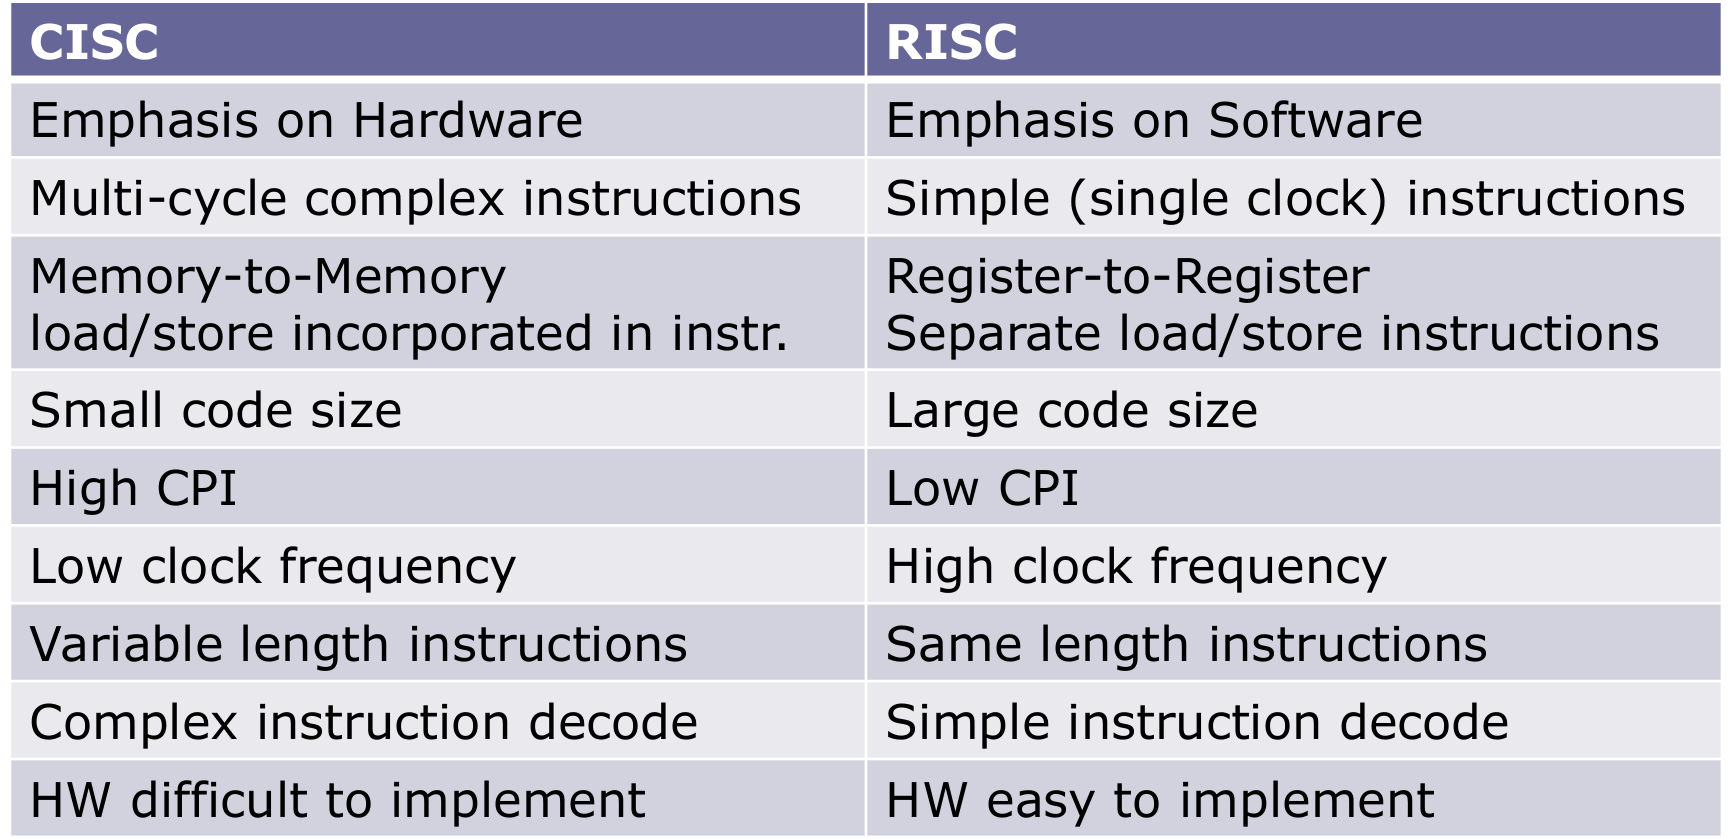
\includegraphics[width=\linewidth]{png/risc.png}
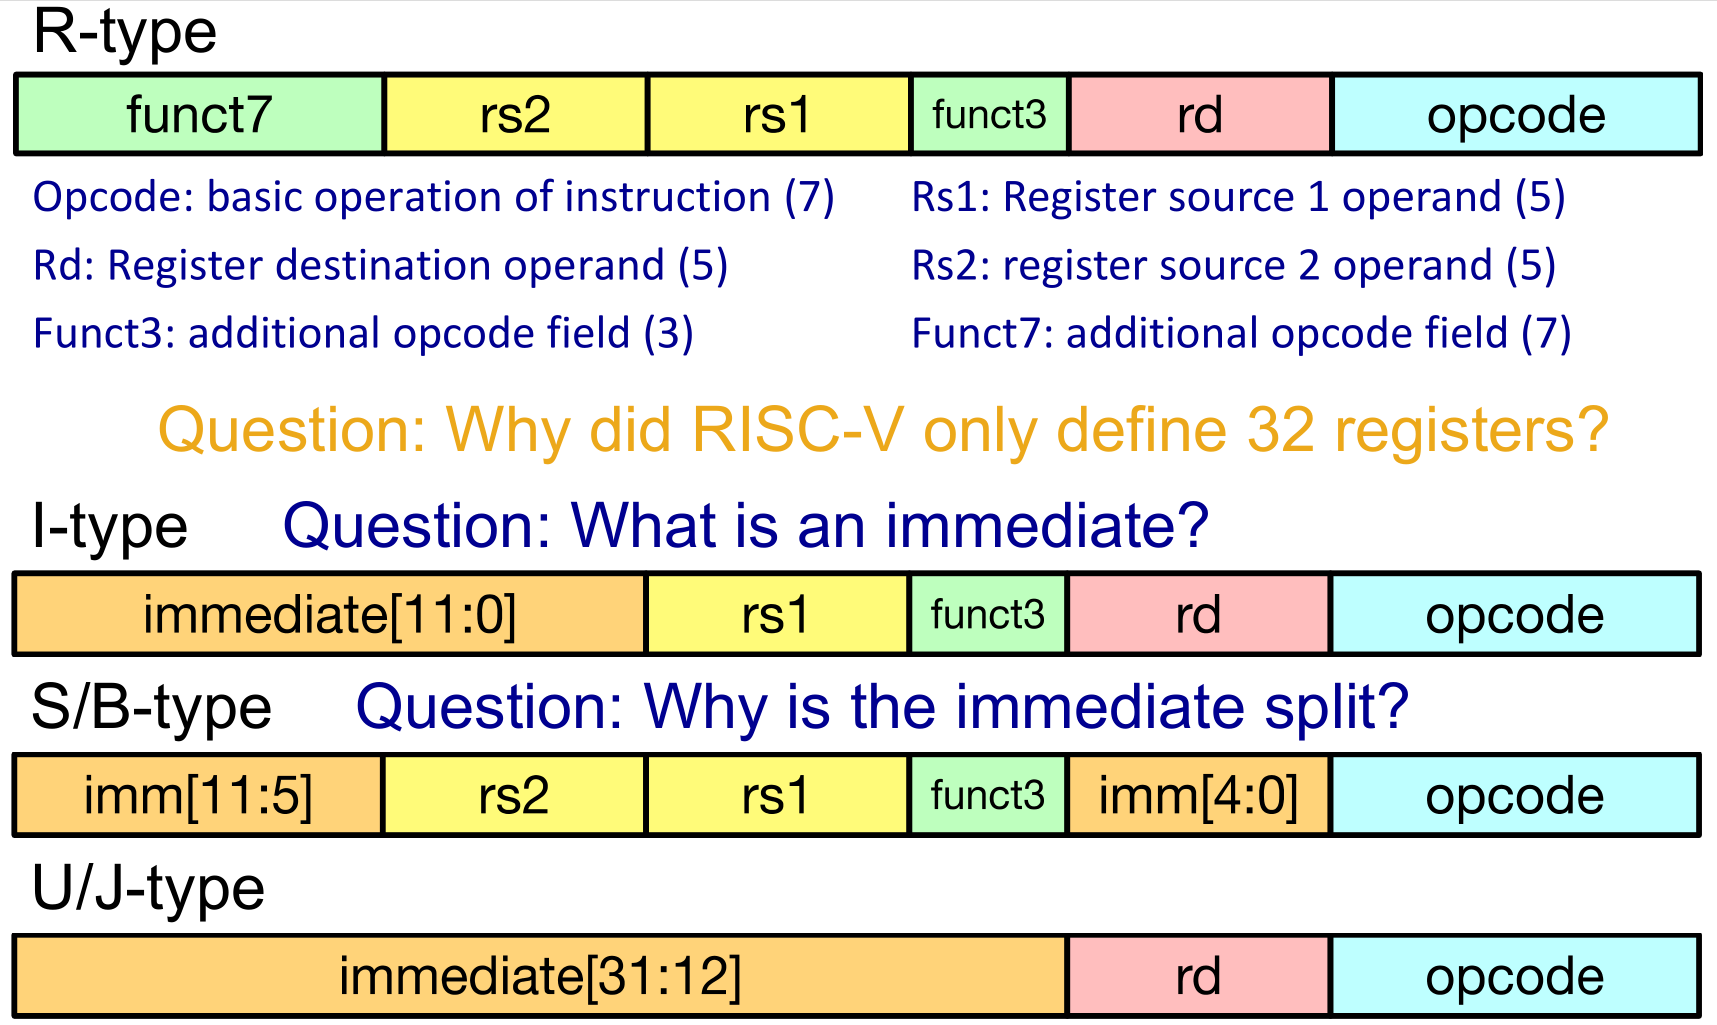
\includegraphics[width=\linewidth]{png/isa.png}

Constant == immediate == literal == offset

There are 32 registers in RISC-V

\textbf{ld dst, offset(base)} the base is the starting address of the array the
offset is the index

When using switch statement we can use a jump table, a jump table holds addresses
in memory of where the code for the jump targets are.

\textbf{Procedures:} are required for structured programming, to implement them
in assembly you need a memory space for local vars, arguments must be passed in
and return values must be passed out, execution must continue after the call.

\textbf{Stack:} The stack is a LIFO data-structure allocated in frames, it
stores the state of a procedure for a limited time, the callee returns before
the caller does. The things which can be saved on the stack are: local arrays,
return addresses, saved registers, and nested call arguments

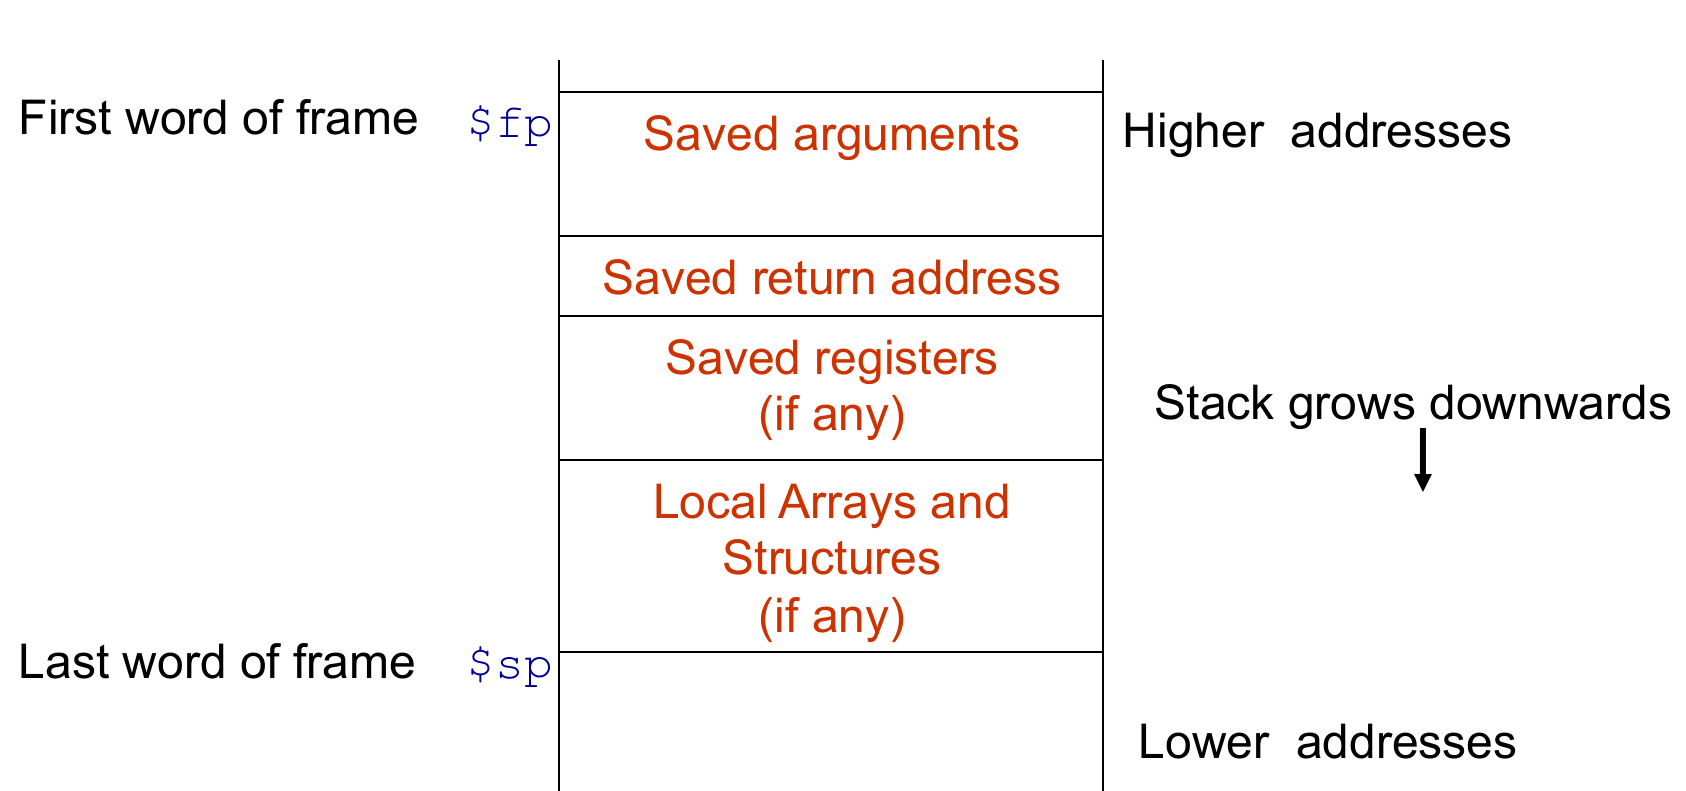
\includegraphics[width=\linewidth]{png/stack.png}
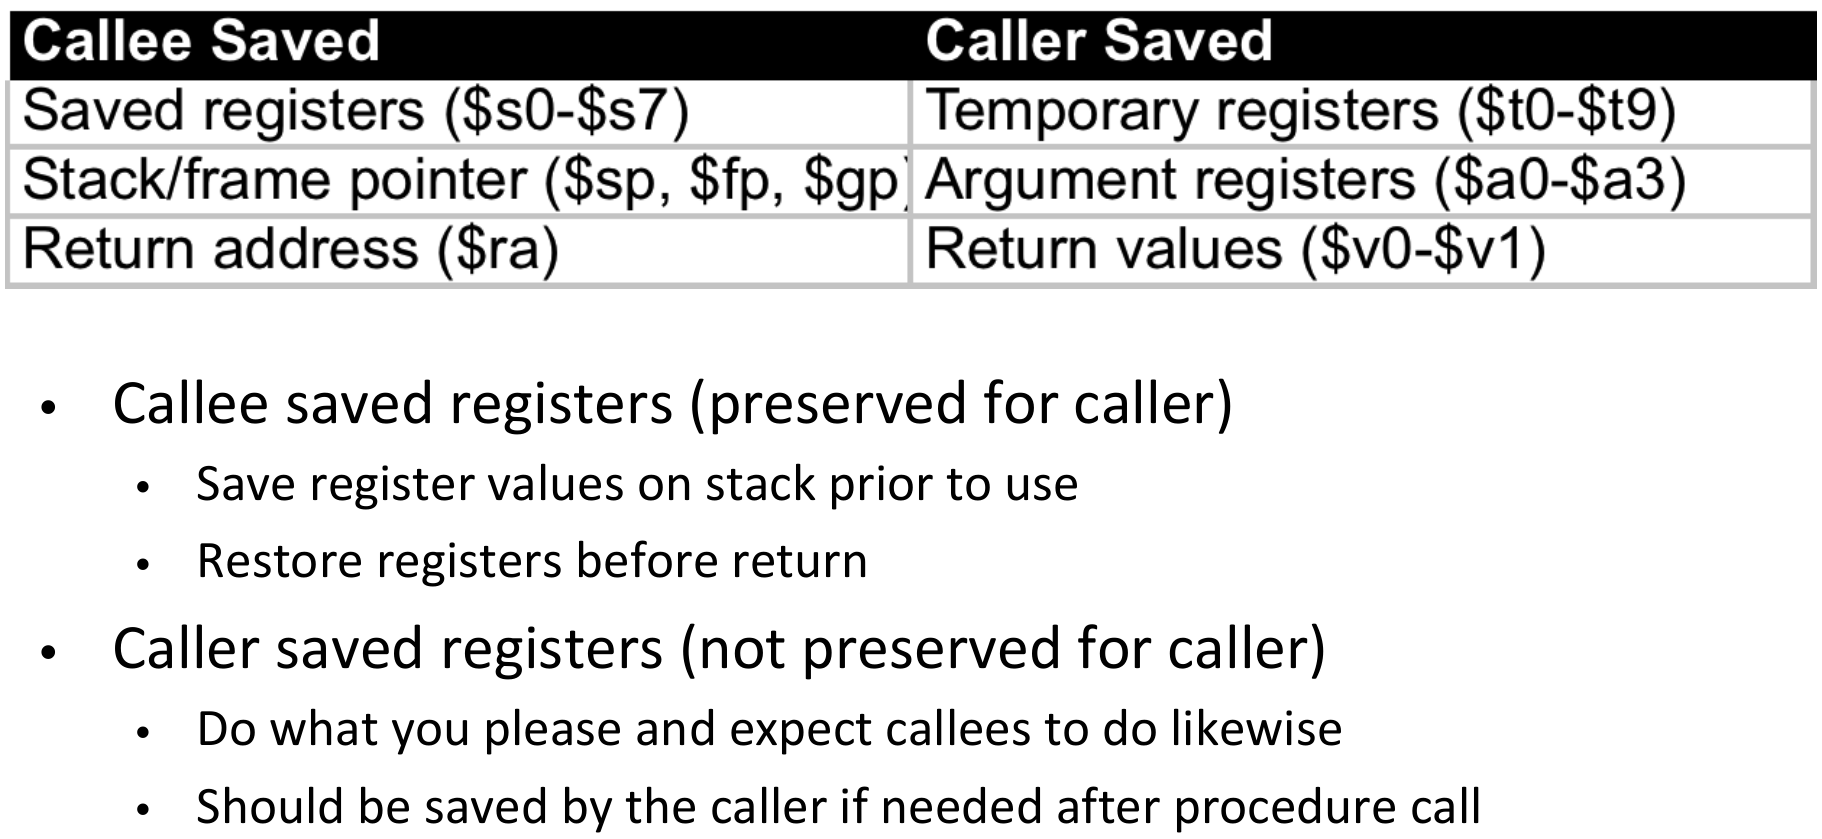
\includegraphics[width=\linewidth]{png/save.png}
\textbf{Procedure Call Steps}
\begin{enumerate}
\item Place parameters in a place where the procedure can access them
\item Transfer control to the procedure
\item Allocate the memory resources needed for the procedure
\item Perform the desired task
\item Place the result value in a place where the calling program can access it
\item Free the memory allocated in (3)
\item Return control to the point of origin
\end{enumerate}
